%
%  Systeemianalyysin laboratorion kandidaatintyön LaTeX-pohja
%  Luonut Juha Törmänen 11.11.2011
%  Päivitetty viimeksi 11.11.2011
%
%  Pohja olettaa, että käytössäsi on kohtuullisen tuore ja hyvin varustettu
%  LaTeX-asennus. Se toimii ainakin Aallon Unix-ympäristössä.
% 
%  Jos teet parannuksia tähän tiedostoon, pyydän ystävällisesti jakamaan
%  ne muiden tekijöiden kanssa - lähetä parannukset joko osoitteeseen
%  juha.tormanen@aalto.fi tai koko parannettu pohja suoraan
%  seminaarista vastaavalle opettajalle.
%
%  Tämän pohjan tuottama ulkoasu pohjautuu Nopasta löytyvään TFM-kandin
%  "Ohje: Kandidaatintyön rakenne ja muotoseikat"-dokumenttiin.
%  https://noppa.aalto.fi/noppa/kurssi/tfm.kand/materiaali
%

% Vaihda kieli jos kirjoitat englanniksi:
\documentclass[a4paper,finnish,titlepage,12pt]{article} 
\usepackage[finnish]{babel}
%\documentclass[a4paper,english,titlepage,12pt]{article} 
%\usepackage[english]{babel}

% Oleellisia paketteja - näiden muuttamiseen tuskin on syytä
\usepackage{amsmath}   % matematiikkaa
\usepackage[utf8]{inputenc} 	% tämä dokumentti on UTF-8-koodattu
\usepackage[T1]{fontenc} 	% tuki ääkkösille
\usepackage{ifpdf}	% PDF-tarkistus
\usepackage{fancyhdr}	% sivunumeron määrittämiseen yläreunaan
\usepackage{parskip}	% kappaleiden väliin rivinvaihto, ei sisennystä
\usepackage{amssymb}



\usepackage[pdftex]{graphicx}   % --> LaTex =>PDF con epstodf
\usepackage{epstopdf}           % --> LaTex =>PDF con epstodf

\usepackage{pdfpages}	% liitä pdf-sivuja dokumenttiin (tiivistelmää varten)
% \usepackage{setspace}	% rivinvälien hallintaan
\usepackage{graphicx}	% Grafiikkatuki

% Linkit, jotka eivät hyppää silmille
\usepackage[pdfpagemode=None, colorlinks=true, urlcolor=blue, linkcolor=black, citecolor=black, pdfstartview=FitH]{hyperref}

%
% VALINNAISET PAKETIT
%  Ota käyttöön allaolevia, jos tarvitset niitä
%  (käyttöönotto: poista %-kommenttimerkki rivin edestä)
%

% Hyödyllisiä matematiikkapaketteja
%  erityisesti: kannattaa käyttää amsmath-paketista löytyvää
%  align-komentoa eqnarrayn sijaan
%\usepackage{amsmath}
%\usepackage{amssymb}
%\usepackage{latexsym}

% Lähdekoodin sisällyttäminen dokumenttiin
%\usepackage{listings}

% Moniosaiset kuvat
%\usepackage{subfig}

% Tekstin sisään sopivat luonnolliset lähdeviittaukset
%  esim. Hämäläinen [2001], [Hämäläinen and Salo 1992]
\usepackage{natbib}






\begin{document}

\ifpdf
\DeclareGraphicsExtensions{.pdf, .jpg, .tif}
\else
\DeclareGraphicsExtensions{.eps, .jpg}
\fi

% Sivunumerointi aloitetaan roomalaisilla numeroilla
%  (nimiölehdellä ei näy sivunumeroa dokumentin titlepage-parametrin vuoksi)
\pagenumbering{roman}
\pagestyle{empty} % piilottaa sivunumerot koko alkuosasta

\begin{titlepage}
	Aalto-yliopisto \\
	Perustieteiden korkeakoulu \\
	Teknillisen fysiikan ja matematiikan tutkinto-ohjelma \\
	% Aalto University \\
	% School of Science \\
	% Degree programme in Engineering Physics and Mathematics \\
	
	\vfill
	
	\begin{center}
		%\begin{spacing}{1.75}
		{\LARGE Ylikerroinstrategiat ja Poisson-mallit vedonlyönnissä}
		%\end{spacing}
		
		Kandidaatintyö \\
		\today

		\vspace{3cm}

		{\large Jussi Kolehmainen}

	\end{center}

	\vfill

	% Jätä kommentoimatta, jos haluat työsi olevan saatavilla verkossa:
	Työn saa tallentaa ja julkistaa Aalto-yliopiston avoimilla verkkosivuilla. \\
	Muilta osin kaikki oikeudet pidätetään.
	% The document can be stored and made available to the public on the open internet pages of Aalto University. \\ 
	% All other rights are reserved.
\end{titlepage}

%
% TIIVISTELMÄPOHJA
%  Lataa tiivistelmäpohja täytettäväksi osoitteesta
%  https://noppa.aalto.fi/noppa/kurssi/tfm.kand/materiaali
%  ja tallenna se PDF-muodossa nimellä tiivistelma.pdf tähän hakemistoon
%

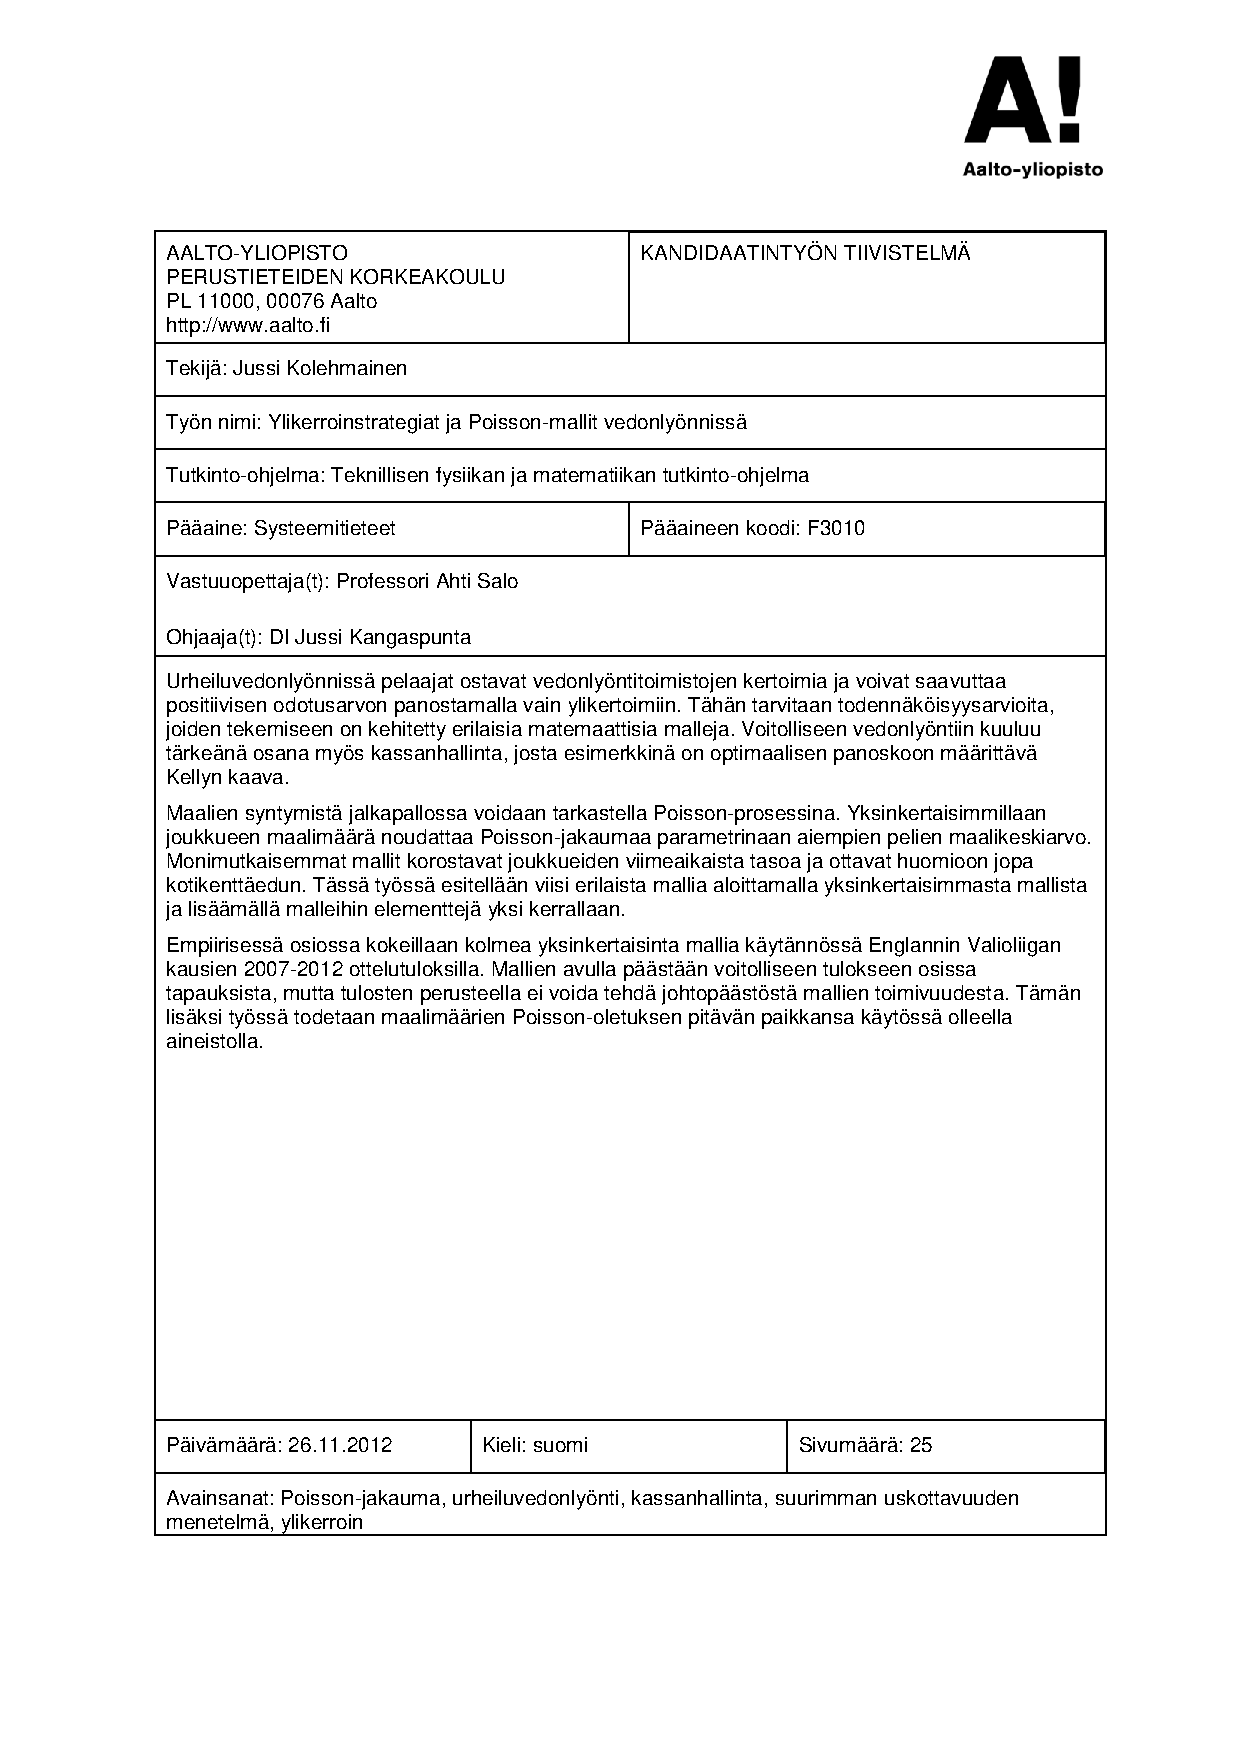
\includepdf{tiivistelma}

% Sisällysluettelo
\tableofcontents
\newpage

% Aloita todellinen sivunumerointi ensimmäisestä sisältösivusta
\pagestyle{fancy}

% Tyhjennetään kentät ja muotoilu
\fancyhf{}
\renewcommand{\headrulewidth}{0pt}
\renewcommand{\footrulewidth}{0pt}

% Sivunnumero ylhäällä oikealla
\rhead{\footnotesize \thepage} 
\pagenumbering{arabic}

% Ensimmäisellä sivulla ei kuitenkaan näytetä numeroa
\thispagestyle{empty} 

% Dokumentin rakenne myötäilee TFM-suosituksia
% --------------------------------------------------------------------


\section{Johdanto}
\subsection{Yleiskuvaus}
Maailmalla käytetään vedonlyöntiin paljon\footnote{Pelkästään Euroopan alueen vedonlyöntimarkkinoiden liikevaihto ylitti 8 miljardia euroa vuonna 2010 \cite{turnover}.} rahaa, mikä on innostanut yhä useampia vedonlyöjiä tutustumaan tarkemmin vedonlyönnin todennäköisyysteoriaan paremman tuloksen toivossa. Useimpien tarkastelujen pohjalla on matemaatikkojen kehittämiä malleja urheilutulosten ennustamiseen. Esimerkiksi jalkapallo-ottelua on lähestyttävä tilastollisin menetelmin, koska se sisältää runsaasti satunnaisia elementtejä. Järjestelmällisen vedonlyönnin tavoitteena on päästä voitolliseen tulokseen yksittäisen ottelun sijaan pitkässä juoksussa, jopa satojen otteluiden jaksoilla.

Jo 1950-luvulla esitettiin mahdollisuus käyttää Poisson-jakaumaa jalkapallo-ottelun maalimäärien mallintamiseen \cite{moroney}. Poisson-jakauma antaa todennäköisyyden tietylle määrälle tapahtumia, tässä tapauksessa maaleille, sillä oletuksella, että satunnaisilmiö on Poisson-jakautunut. Tätä ideaa on vuosikymmenten kuluessa viety eteenpäin luomalla Poisson-jakaumaan perustuvia monimutkaisempia malleja, jotka kuvaavat paremmin maalintekoprosessin käyttäytymistä.

Tässä työssä tutustutaan muutamiin näistä malleista ja kokeillaan käytännössä kolmea yksinkertaisinta oikeilla ottelutuloksilla. Tämän lisäksi testataan oletusta, jonka mukaan maalimäärät ovat Poisson-jakautuneet. Työn tavoitteena on saada tarkasteltavista malleista käyrä, joka kuvaa pelikassan kehitystä viiden eri kauden keskiarvona. Tällä pyritään löytämään onko yksinkertaisilla mallilla mahdollista päästä voitolliseen vedonlyöntiin pitkällä aikavälillä. 
Lisäksi mallien antamia tuloksia verrataan satunnaisen vedonlyönnin tuloksiin.






\subsection{Työn rakenne}
Kappaleessa 2.1 annetaan perustietoa 1X2-vedonlyöntimuodosta, johon tämä työ keskittyy. Kappaleissa 2.2 ja 2.3 esitellään kertoimien merkitys ja mahdollisuus positiiviseen palautuksen odotusarvoon ylikertoimien avulla. Kappaleessa 2.4 kuvaillaan kassanhallintaa ja strategiaa empiiristä osiota varten.

Kappaleessa 3 tutustutaan matemaattisiin malleihin, joiden avulla määritetään todennäköisyysjakaumia jalkapallo-otteluiden päättymisvaihtoehdoille. Kappaleissa 3.1 ja 3.2 määritellään Poisson-jakauma ja esitetään koeasetelma Poisson-jakaumaoletuksen testaamiseksi.  Kappaleissa 3.3 - 3.7 esitellään todennäköisyysmalleja, jotka kaikki pohjautuvat Poisson-jakaumaan.

Kappale 4 on empiirinen osio, jossa malleja testataan käytännössä vanhoilla ottelutuloksilla. Kappaleessa 4.1 määritellään koeasetelma ja käytettävät menetelmät. Kappaleissa 4.2 ja 4.3 kuvataan teknistä toteutusta ja kokeiden suoritusta. Kappaleessa 4.4 esitetään ja analysoidaan saatuja tuloksia.

Kappaleessa 5 käydään läpi yhteenveto ja esitetään mahdollisia jatkotutkimuksen aiheita.

\section{Vedonlyöntiteoriaa}
\subsection{1X2-veikkaus}
Jalkapallo-ottelulla on kolme mahdollista päättymisvaihtoehtoa: kotivoitto, tasapeli ja vierasvoitto. Näitä merkitään yleisesti merkeillä 1, X ja 2. Tässä työssä keskitytään vain normaaleihin sarjapeleihin, jotka loppuvat aina 90 minuutin (ja muutaman minuutin lisäajan) jälkeen johonkin näistä kolmesta vaihtoehdosta.

Työssä tarkastellaan vedonlyöntiä, jossa pelaajat pelaavat vedonlyöntitoimistoa vastaan. Vedonlyöntitoimisto tarjoaa kertoimia $o_1$, $o_X$ ja $o_2$ kotivoitolle, tasapelille ja vierasvoitolle (o = odds, $o_i > 1.0$). Pelaaja asettaa panoksensa $b_i$ (b = bet) merkille $i$. Mikäli ottelu päättyy pelaajan veikkaamaan merkkiin $i$, maksaa toimisto pelaajalle palautuksen (R = return)
\begin{equation}
R = o_i \cdot b_i.
\end{equation}
Ottelun päättyeessä muihin merkkeihin pelaajalle ei palauteta mitään. Osuessaan oikeaan merkkiin pelaaja jää voitolle summan $o_i \cdot b_i - b_i = (o_i - 1) \cdot b_i$.

\subsection{Mistä kertoimet tulevat?}
Merkitään edelleen vedonvälittäjän tarjoamia kertoimia $o_1$, $o_X$ ja $o_2$. Oletetaan, että todelliset todennäköisyydet merkeille ovat $p_1$, $p_X$ ja $p_2$ (p = probability), joille pätee $p_1 + p_X + p_2 = 1$. Huomioitavaa on, että tässä ei oteta kantaa siihen, saadaanko näitä todennäköisyyksiä selville mistään. Oletetaan ainoastaan, että todennäköisyydet ovat olemassa.

Vedonlyöntitoimisto käyttää kertoimien määrittämiseen useita eri menetelmiä \cite{odds}:

\begin{enumerate}
  \item Todennäköisyysarviot
  \item Pelaajien odotettu panosjakauma
  \item Asiantuntija-arviot
\end{enumerate}

Periaatteessa kertoimet saadaan asettamalla voiton odotusarvo nollaksi:
\begin{eqnarray}
&& E[R] = p o b - b = (p o - 1) b = 0 \\
&\Leftrightarrow& o = 1 / p,
\end{eqnarray}

missä $p$ on toimiston todennäköisyysarvio, $o$ kerroin ja $b$ panoksen suuruus. Vedonlyöntitoimisto ottaa kuitenkin pelivaihdosta komission, jonka vaikutuksesta kertoimet ovat tätä pienempiä. Todellisuudessa siis toimisto määrittää kertoimet niin, että $o < 1 / p$. Toimisto käyttää todennököisyyksien määrittämiseen erilaisia laskennallisia menetelmiä, joista muutamia esimerkkejä tarkastellaan tämän työn kappaleessa 3.

Jos toimisto määrittäisi kertoimet pelkästään todennäköisyysarvioiden perusteella, se jäisi odotusarvoisesti tappiolle, koska suurin osa pelaajista ei pelaa tämän jakauman mukaisesti. Useimmat harrastelijavedonlyöjät panostavat järkisyiden sijaan tunnesyistä, kuten esimerkiksi oman suosikkijoukkueensa puolesta. Toimisto ottaa huomioon pelaajien odotetun panostuskäyttäytymisen ja asettaa paljon pelattaville merkeille pienemmät kertoimet. Toimisto muuttaa usein kertoimiaan ottelun lähestyessä, jos panosjakauma ei ole odotetunlainen. Näin se varmistaa itselleen mahdollisimman suuren voiton odotusarvon.

Ottelun lopputulokseen vaikuttavat myös yksittäiset tekijät, kuten loukkaantumiset ja väsymys, joita laskennallisten menetelmien on hyvin vaikea ottaa huomioon. Näiden tekijöiden huomioonottamiseksi toimisto käyttää myös lajikohtaisia asiantuntijoita kertoimien määritykseen.


\subsection{Ylikertoimet}
Koska toimiston kertoimet $o_1$, $o_X$ ja $o_2$ eivät välttämättä vastaa todellisista todennäköisyyksistä $p_1$, $p_X$ ja $p_2$ johdettuja kertoimia, pelaaja voi löytää tilanteita, joissa se pääsee odotusarvoisesti voitolle. Olkoon $b$ pelaajan asettama panos kertoimella $o$, jonka todellinen todennäköisyys on $p$. Pelaaja voittaa summan $ob$ todennäköisyydellä $p$ ja menettää alkuperäisen panoksen varmasti. Tällöin palautuksen $R$ odotusarvo on positiivinen, kun

\begin{eqnarray}
	&& E[R] = (p o - 1) b > 0 \\
	&\Leftrightarrow& o > 1 / p.
\end{eqnarray}

Tämä voidaan tulkita niin, että toimiston tarjoama kerroin on todennäköisyyteen nähden liian suuri. Pelaaja voi hyödyntää tämän laskemalla omat todennäköisyysarviot $p_{i}^{P}$ (P = player), joille pätee mahdollisimman tarkasti $p_{i}^{P} \approx p_i$. Tämän jälkeen pelaajan on etsittävä vedonlyöntitoimiston listoilta kohteita, joille pätee yhtälö (5). Panostaminen tähän merkkiin kannattaa, koska arvion mukaan palautuksen odotusarvo on positiivinen.

\subsection{Panostaminen ja kassan kasvunopeus}
Kun sopiva ylikerroin on löydetty, on seuraava vaihe löytää optimaalinen summa, joka merkkiin panostetaan. Tähän kysymykseen odotusarvon maksimoiminen ei ole sopiva ratkaisu, sillä sen mukaan olisi panostettava aina koko kassa. Tämä johtaa siihen, että koko pelikassa hävitään suurella todennäköisyydellä \cite{growth}.

Odotusarvon maksimoimisen sijaan on maksimoitava pelikassan kasvunopeutta. Seuraavassa johdetaan lauseke pelikassan kasvunopeudelle ja sen maksimoivalle panoskoolle \cite{kelly}.

Olkoon pelaajan pelikassa $k$:n peräkkäisen vedon jälkeen $B_k$.  Olkoon $s \in [0,1]$ osuus, joka panostetaan seuraavaan vetoon pelikassasta. Merkitään edelleen kohteen kerrointa $o$ ja todennäköisyyttä $p$. Mikäli veto voitetaan, on uusi pelikassan koko
\begin{equation}
	B_{1} = B_0 + osB_0 - sB_0 = (1 + (o-1)s) B_0
\end{equation}

ja hävittäessä
\begin{equation}
	B_{1} = B_0 - sB_0 = (1 - s) B_0.
\end{equation}

Oletetaan, että $N$:sta peräkkäisestä vedosta voitetaan $W$ ja hävitään $L$ kappaletta. Tällöin
\begin{equation}
	B_{N} = (1 + (o-1)s)^{W} \cdot (1 - s)^{L} \cdot B_{0}.
\end{equation}

Kasvunopeuden geometrinen keskiarvo $G$ vetoa kohden saadaan ottamalla $N$:s juuri edellisen lausekkeen kertoimesta. Tällöin
\begin{eqnarray}
	E[G] &=& (1 + (o-1)s)^{W/N} \cdot (1 - s)^{L/N} \\
	&\approx& (1 + (o-1)s)^p \cdot (1 - s)^{1-p},
\end{eqnarray}

koska suurilla $N$ pätee $W/N \approx p$ ja $L/N \approx 1-p$. Maksimoidaan $G$ panostusosuuden $s$ suhteen maksimoimalla sen logaritmia
\begin{eqnarray}
	\alpha &=& ln (E[G]) \\
	&=& p \cdot ln(1+(o-1)s) + (1-p) \cdot ln(1-s).
\end{eqnarray}

Maksimi löytyy derivaatan nollakohdasta:

\begin{eqnarray}
	&\frac{\partial \alpha}{\partial s}& = \frac{p(o-1)}{1+(o-1)s} - \frac{1-p}{1-s} = 0 \\
	&\Leftrightarrow& s(o-1) = po - 1 \\
	&\Leftrightarrow& s = \frac{po-1}{o-1}.
\end{eqnarray}

Tuloksena on kuuluisa Kellyn kaava, jota käytetään myös taloustieteessä sijoituskohteiden arviointiin. Usein käytetään lisäksi Kellyn jakajaa, jolloin panoskoko on vain osa edellisestä kaavasta. Mitä suurempi jakaja on, sitä pienempi on volatiliteetti eli kassan suuruuden vaihtelu \cite{divider}.

\section{Poisson-jakaumaan perustuvia malleja}

\subsection{Poisson-jakauma}
Poisson-jakauma on diskreetti todennäköisyysjakauma, joka liittää todennäköisyyden tapahtumien lukumäärään kiinteällä aikavälillä, kun tapahtumat ovat riippumattomia ja niiden lukumäärän odotusarvo on vakio. Merkintä satunnaismuuttujalle $X$ on
\begin{equation}
	X \sim Poisson(\lambda),
\end{equation}

missä $\lambda > 0$ on intensiteetti. Jakauman odotusarvo on $E[X] = \lambda$ ja varianssi $Var[X] = \lambda$. Pistetodennäköisyysfunktio Poisson-jakaumalle on
\begin{equation}
	P(X = k) = e^{-\lambda} \frac{\lambda^k}{k!}, \; k \in \mathbb{Z}_{+} \cup \{0\}.
\end{equation}

Ylikertoimien löytämiseksi on määritettävä todennäköisyydet eri päätösvaihtoehdoille 1, X ja 2. Kappaleissa 3.2 ja 3.3 pohditaan Poisson-jakauman sopivuutta jalkapallo-ottelun mallintamiseen. Kappaleissa 3.4 - 3.7 esitetään Poisson-jakaumaan perustuvia malleja jalkapallo-ottelun todennäköisyysjakauman määrittämiseksi.


\subsection{Ovatko maalimäärät Poisson-jakautuneita?}
Pearsonin $\chi^2$-testiä voidaan käyttää testaamaan ovatko havaitut frekvenssit peräisin jostain tietystä todennäköisyysjakaumasta \cite{mellin}. Merkitään havaittuja frekvenssejä $O_i$, $i=1, 2, ..., n$. Teoreettiset frekvenssit $E_i$ saadaan kyseessä olevan jakauman $P$ avulla
\begin{equation}
	E_i = n \cdot P(x = i).
\end{equation}

Testin hypoteeseinä ovat
\begin{eqnarray*}
	&H_0&: \text{ Frekvenssit noudattavat kyseessä olevaa jakaumaa} \\
	&H_1&: \text{ Frekvenssit eivät noudata kyseessä olevaa jakaumaa}.
\end{eqnarray*}

Käytettävä testisuure saadaan
\begin{equation}
	\chi^2 = \sum_{i=1}^{n} \frac{(O_i - E_i)^2}{E_i},
\end{equation}

ja se noudattaa nollahypoteesin ollessa voimassa $\chi^2$-jakaumaa vapausastein $k - p - 1$, missä $k$ on frekvenssiluokkien määrä ja $p$ on havainnoista estimoitujen parametrien määrä.


Tässä tapauksessa testataan ovatko yksittäisen joukkueen maalimäärät kauden aikana yhteensopivia Poisson-jakauman kanssa. Poisson-jakauman parametrin suurimman uskottavuuden estimaatti saadaan joukkueen koko kauden maalimääristä (kappale 3.4).  Tässä tapauksessa $k = 6$ jos viidennen maalin jälkeen tulevia maaleja ei huomioida ja $p = 1$, koska ainut esimoitava parametri on Poisson-jakauman parametri.

Viidennen maalin jälkeen tulevat maalit hylätään, koska ne rikkovat Poisson-jakauman oletuksen, että uudet maalit olisivat riippumattomia aikaisemmista. Näin suurissa maalimäärissä tappiolla olevan joukkue menettää motivaationsa kokonaan, ja uusia maaleja voi syntyä lisää riippumatta joukkueiden taitotasoista.


\subsection{Maalijakauman hyödyntäminen}
Tässä työssä esiteltävät mallit perustuvat joukkueiden maalimäärien mallintamiseen Poisson-jakauman muunnelmien avulla. Työssä keskitytään kuitenkin ainoastaan 1X2-vedonlyöntiin, joten tulosjakauma on muunnettava jakaumaan, joka sisältää ainoastaan kotivoiton, tasapelin ja vierasvoiton todennäköisyyden.

Merkin $i$ todennäköisyysarvio saadaan
\begin{equation}
	p_{i}^{P} = \sum_{j,k \in U_i} P(X=j, Y=k),
\end{equation}

missä
\begin{eqnarray*}
	U_1 &=& \{(j,k)|j>k\} \\
	U_X &=& \{(j,k)|j=k\} \\
	U_2 &=& \{(j,k)|j<k\}.
\end{eqnarray*}

Kotivoiton todennäköisyys saadaan siis summaamalla kaikkien kotivoittotulosten todennäköisyydet. Vastaavasti saadaan todennäköisyydet myös tasapelille ja vierasvoitolle. Maalimäärille voidaan olettaa jokin yläraja, esimerkiksi edellä käytetty 5 maalia, jotta summattavien termien määrä saadaan äärelliseksi.



\subsection{Jalkapallo-ottelun mallinnus Poisson-jakaumalla}
Moroney \cite{moroney} oletti koti- ja vierasjoukkueen maalimäärien X ja Y noudattavan riippumattomia Poisson-jakaumia parametrein $\lambda$ ja $\mu$.
Tällöin tuloksen (x, y) todennäköisyys saadaan
\begin{equation}
	P(X = x, Y = y) = \frac{\lambda^x e^{-\lambda}}{x!} \cdot \frac{\mu^y e^{-\mu}}{y!}.
\end{equation}

Parametrit $\lambda$ ja $\mu$ saadaan estimoitua aikaisemmista ottelutuloksista suurimman uskottavuuden menetelmällä. Maalimäärien riippumattomuuden vuoksi esimointi voidaan suorittaa joukkuekohtaisesti aikaisemmista otteluista. Olkoon aineistona $n$ kappaletta kotijoukkueen pelattuja otteluita maalimäärillä $x_1, x_2, ..., x_n$. Tällöin logaritminen suurimman uskottavuuden funktio kotijoukkueelle on
\begin{eqnarray}
	\log{L(\lambda)} &=& \log{\prod_{i=1}^{n} \frac{\lambda^{x_i} e^{-\lambda}}{x_i!}} \\
	&=& \sum_{i=1}^{n} (x_i \log{\lambda} - \lambda + \log{x_i!}).
\end{eqnarray}

Maksimi löydetään logaritmisen uskottavuusfunktion derivaatan nollakohdasta.
\begin{eqnarray}
	\frac{\partial}{\partial \lambda} \log{L(\lambda)} &=& \sum_{i=1}^{n} (x_i / \lambda - 1) \\
	&=& 1 / \lambda \sum_{i=1}^{n} x_i - n = 0 \\
	\Rightarrow \lambda &=& \frac{1}{n} \sum_{i=1}^{n} x_i.
\end{eqnarray}

Suurimman uskottavuuden estimaattori parametrille on siis keskiarvo edellisten otteluiden tehdyistä maaleista. 

\subsection{Puolustus- ja hyökkäysparametrit}
Maher \cite{maher} vei Moroneyn mallia eteenpäin asettamalla joukkueille hyökkäys- ja puolustusparametrit, joista Poisson-jakauman intensiteetti riippuu. 

Merkitään kotijoukkueen hyökkäystä ja puolustusta parametreillä $\alpha_i$ ja $\gamma_i$. Vastaavasti vierasjoukkueelle merkitään $\delta_j$ ja $\beta_j$. Nyt voidaan merkitä koti- ja vierasjoukkueiden maalimääriä
\begin{eqnarray}
	X_{ij} &\sim& Poisson(\alpha_i \beta_j) \\
	Y_{ij} &\sim& Poisson(\gamma_i \delta_j).
\end{eqnarray}

Sarjassa, jossa on $n$ joukkuetta, on yhteensä $4n$ estimoitavaa parametria. Kuitenkin parametrit voidaan skaalata niin, että on voimassa
\begin{eqnarray}
	\sum_{i=1}^{n} \alpha_i &=& \sum_{j=1}^{n} \beta_j \\
	\sum_{i=1}^{n} \gamma_i &=& \sum_{j=1}^{n} \delta_j.
\end{eqnarray}

eli riippumattomia parametrejä on $4n - 2$ kappaletta. Satunnaismuuttujien $X_{ij}$ ja $Y_{ij}$ riippumattomuudesta seuraa se, että parametrit $\alpha_i$ ja $\beta_j$ estimoidaan vain kotijoukkueiden maalimäärien $x_{ij}$ avulla. Vastaavasti $\gamma_i$ ja $\delta_j$ saadaan vierasjoukkueiden maalimäärien $y_{ij}$ avulla.

Suurimman uskottavuuden funktio parametrijoukoille $\mathbf{\alpha}$ ja $\mathbf{\beta}$ on
\begin{eqnarray*}
	L(\mathbf{\alpha}, \mathbf{\beta}) &=& P(X_{ij}=x_{ij} \forall i,j=1,...,n | \mathbf{\alpha}, \mathbf{\beta}) \\
	&=& \prod_{i,j \ne i} \frac{(\alpha_i \beta_j)^x_{ij}}{x_{ij}!} e^{-\alpha_i \beta_j}.
\end{eqnarray*}

Ottamalla tästä logaritmi saadaan edelleen
\begin{eqnarray*}
	\log{L(\mathbf{\alpha}, \mathbf{\beta})} &=& \sum_{i} \sum_{j \ne i} (-\alpha_i \beta_j + x_{ij} \log{\alpha_i \beta_j) - log(x_{ij}!}).
\end{eqnarray*}

Logaritmisesta uskottavuusfunktiosta otetaan derivaatta parametrien suhteen, jolloin saadaan

\begin{eqnarray*}
	\frac{\partial \log{L}}{\partial \alpha_i} &=& \sum_{j \ne i} (-\beta_j + \frac{x_{ij}}{\alpha_i}) \\
	\frac{\partial \log{L}}{\partial \beta_j} &=& \sum_{i \ne j} (-\alpha_i + \frac{x_{ij}}{\beta_j}).
\end{eqnarray*}

Suurimman uskottavuuden estimaattorit $\hat{\alpha}_i$ ja $\hat{\beta}_j$ saadaan merkitsemällä derivaatat nolliksi, jolloin saadaan yhtälöt

\begin{eqnarray*}
	\hat{\alpha}_i &=& \frac{\sum_{j \ne i} x_{ij}}{\sum_{j \ne i} \hat{\beta}_j} \\
	\hat{\beta}_j &=& \frac{\sum_{i \ne j} x_{ij}}{\sum_{i \ne j} \hat{\alpha}_i}.
\end{eqnarray*}

Yhtälöryhmä saadaan ratkaistua numeerisesti laskemalla vuorotellen hyökkäysparametrit puolustusparametrien avulla ja toisinpäin. Iteraation alkuarvoiksi Maher suosittelee arvoja
\begin{eqnarray}
	\hat{\alpha}_i^0 &=& \sum_{j \ne i} \frac{x_{ij}}{\sqrt{S_X}} \\
	\hat{\beta}_j^0 &=& \sum_{i \ne j} \frac{x_{ij}}{\sqrt{S_X}},
\end{eqnarray}

missä $S_X = \sum_{i} \sum_{j \ne i} x_{ij}$.

Vastaavasti käyttämällä vierasjoukkueiden maaleja $y_{ij}$ saadaan estimoitua parametrit $\mathbf{\gamma}$ ja $\mathbf{\delta}$.



\subsection{Korjaustermit tietyille tuloksille}
Dixon ja Coles \cite{dixoncoles} tutkivat maalimäärien Poisson-oletusta ja päätyivät johtopäätökseen, että Poisson-jakauma aliarvioi vähämaalisten (0, 0), (0, 1), (1, 0) ja (1, 1) otteluiden todennäköisyyksiä. 

Dixon ja Coles kehittivät mallin, joka perustuu edellisen kappaleen Maherin malliin, mutta lisää siihen painotustermejä vähämaalisille tuloksille. Tämän lisäksi se huomioi paremmin kotiedun merkitystä jalkapallossa. Malli jakautuu kahteen versioon, joista ensimmäinen olettaa joukkueiden parametrit muuttumattomiksi, ja toinen esittää menetelmiä parametrien päivittämiseen kauden aikana.

\subsubsection{Staattinen malli}
Malli yksinkertaistaa Maherin mallia siten, että jokaisella joukkueella on vain yksi hyökkäys- ja puolustusparametri. Maherin mallissa jokaisella joukkueella on erilliset parametrit koti- ja vierasotteluihin. Dixon ja Coles tuovat malliin kotiedun merkityksen erillisellä kotietuparametrilla $\gamma > 0$. Koti- ja vierasjoukkueen maalimäärien oletetaan noudattavan jakaumia
\begin{eqnarray*}
	X_{ij} &\sim& Poisson(\alpha_i \beta_j \gamma) \\
	Y_{ij} &\sim& Poisson(\alpha_j \beta_i),
\end{eqnarray*}

missä $\alpha$:t kuvaavat joukkueiden hyökkäystä ja $\beta$:t puolustusta.

Kokonaisuudessaan tuloksen (x, y) todennäköisyys on
\begin{equation}
	P(X_{ij}=x, Y_{ij}=y) = \tau_{\lambda,\mu} (x, y) \frac{\lambda^x e^{-\lambda}}{x!} \cdot \frac{\mu^y e^{\mu}}{y!},
\end{equation}

missä $\lambda = \alpha_i \beta_j \gamma$, $\mu = \alpha_j \beta_i$ ja 
\begin{equation}
\tau_{\lambda,\mu} (x, y) =
\begin{cases}
1 - \lambda \mu \rho, & \text{jos } x = y = 0 \\
1 + \lambda \rho, & \text{jos } x = 0, y = 1 \\
1 + \mu \rho, & \text{jos } x = 1, y = 0 \\
		1 - \rho, & \text{jos } x = y = 1 \\
		1, & \text{muuten}.
	\end{cases}
\end{equation} 

Riippuvuusparametrille $\rho$ pätee
\begin{equation}
	max(-1/\lambda, -1/\mu) \le \rho \le max(1/\lambda \mu, 1).
\end{equation}

Malli sisältää $n$ kappaletta hyökkäys- ja puolustusparametrejä $\alpha$ ja $\beta$ sekä riippuvuusparametrin $\rho$ ja kotietuparametrin $\gamma$ eli yhteensä $2n+2$ parametria. Parametreille voidaan asettaa rajoitus

\begin{equation}
	\frac{1}{n} \sum_{i=1}^{n} \alpha_i = 1,
\end{equation}

jolloin estimoitavia parametrejä on $2n+1$ kappaletta.

Mallin uskottavuusfunktioksi saadaan
\begin{equation}
	L(\alpha_i, \beta_i, \rho, \gamma; i=1,...,n) = \prod_{k=1}^{N} \tau_{\lambda_k, \mu_k} (x_k, y_k) e^{-\lambda_k - \mu_k} \lambda_k^{x_k} 			\mu_k^{y_k}
\end{equation}

missä $\lambda_k = \alpha_{i(k)} \beta_{j(k)} \gamma$ ja $\mu_k = \alpha_{j(k)} \beta_{i(k)}$. Tässä indeksit $i(k)$ ja $j(k)$ viittaavat ottelun $k$ koti- ja vierasjoukkueeseen.

Dixon ja Coles ehdottavat uskottavuusfunktion maksimin ratkaisua suoraan numeerisesti. Tätä he perustelevat sillä, että parametrien yhdistelmät ovat lähes ortogonaalisia.
Tässä työssä parametrit ratkaistaan gradienttimenetelmällä, jonka pseudokoodi saatiin viitteen \cite{olesen} sivulta 48.




\subsubsection{Dynaaminen malli}
Todellisuudessa joukkueiden tasot vaihtelevat kauden edetessä ja näin ollen hyökkäys- ja puolustusparametrejä on päivitettävä jatkuvasti. 
Lisäksi huomionarvoista on se, että pääsääntöisesti seuraava ottelu muistuttaa enemmän muutamaa aikaisempaa ottelua kuin esimerkiksi kauden alussa pelattuja otteluita. Tämä voidaan ottaa huomioon mallissa kahdella tapaa.

Ensimmäinen tapa perustuu stokastiseen malliin, jossa parametrit kehittyvät ajassa sisältäen satunnaisuutta. Helpompi tapa on kuitenkin ottaa malliin mukaan funktio, joka painottaa edellisten pelien informaatiota aikaisempia enemmän.

Merkitään painotusfunktiota
\begin{equation}
	\phi (t) = e^{-\xi t}, \; \xi > 0.
\end{equation}

Dynaamisen mallin uskottavuusfunktio on nyt

\begin{equation}
	L(\alpha_i, \beta_i, \rho, \gamma; i=1,...,n) = \prod_{k=1}^{N} \{\tau_{\lambda_k, \mu_k} (x_k, y_k) e^{-\lambda_k - \mu_k} \lambda_k^{x_k} 		\mu_k^{y_k}\}^{\phi(t - t_k)}.
\end{equation}

Staattinen malli saadaan erikoistapauksena, kun $\xi = 0$. Parametrin $\xi$ arvon kasvaessa painotetaan viimeisimpiä pelejä enemmän.

Merkitään kappaleen 3.3 mukaisesti ottelulle $k$ laskettuja todennäköisyyksiä $p_{k,1}$, $p_{k,X}$ ja $p_{k,2}$, jotka saadaan kaavasta (39) suurimman uskottavuuden estimaatteina. Pelkästään näitä todennäköisyyksiä hyödyntäväksi log-likelihood-funktioksi $S(\xi)$ saadaan

\begin{equation}
S(\xi) = \sum_{k=1}^{n} (\delta_{k,1} \log p_{k,1} + \delta_{k,X} \log p_{k,X} + \delta_{k,2} \log p_{k,2}),
\end{equation}

missä 
\begin{equation}
	\delta_{k,i} = 
	\begin{cases}
		1, & \text{jos ottelu k päättyy merkkiin i} \\
		0, & \text{muuten}.
	\end{cases}
\end{equation}

Maksimoimalla funktiota $S(\xi)$ löydetään optimaalinen $\xi$:n arvo.
Tässä työssä ei tarkastella tätä mallia tämän pidemmälle.



\subsection{Kaksimuuttujainen Poisson-jakauma}
Karlis ja Ntzoufras \cite{bivariate} esittivät otteluiden mallinnukseen jakauman, jossa joukkueiden maalimäärät ovat riippuvia. Malli on kaksimuuttujainen Poisson-jakauma, jonka reunajakaumat ovat kuitenkin tavallisia Poisson-jakaumia.

Oletetaan, että satunnaismuuttujat $X_\kappa$, $\kappa = 1,2,3$ noudattavat Poisson-jakaumia parametreilla $\lambda_\kappa$. Tällöin muuttujat $X = X_1 + X_2$ ja $Y = X_2 + X_3$ noudattavat yhdistettyä kaksimuuttujaista Poisson-jakaumaa $BP(\lambda_1, \lambda_2, \lambda_3)$, jolle pätee
\begin{equation}
	P(X=x, Y=y) = e^{-(\lambda_1 + \lambda_2 + \lambda_3)} \sum_{k=0}^{min(x,y)} \binom{x}{k} \binom{y}{k} k! (\frac{\lambda_3}{\lambda_1 \lambda_2})^k.
\end{equation}

Reunajakaumille pätee $E[X] = \lambda_1 + \lambda_2$ ja $E[Y] = \lambda_2 + \lambda_3$ ja maalimäärien koveranssi on $Cov(X,Y) = \lambda_3$. Parametrit voidaan tulkita niin, että $\lambda_1$ ja $\lambda_2$ kuvaavat joukkueiden maalintekokykyä kun taas $\lambda_3$ kuvaa ottelutapahtumia ja olosuhteita.

Kaksimuuttujaisen Poisson-jakauman tapauksessa helpoin tapa siirtyä tulosjakaumasta 1X2-jakaumaan on laskea joukkueiden maalien erotus $Z = X - Y$:

\begin{equation}
P(Z=z) = e^{-(\lambda_1 + \lambda_2)} (\frac{\lambda_1}{\lambda_2})^{z/2} I_z (2\sqrt{\lambda_1 \lambda_2}),
\end{equation}

missä $z = -3,2,...2,3$ ja $I_Z$ on Besselin funktio
\begin{equation}
	I_r (x) = (\frac{x}{2})^r \sum_{k=0}^{\infty} \frac{(x^2/4)^k}{k! \cdot \Gamma(r + k + 1)}.
\end{equation}

Kotivoiton todennäköisyys saadaan tästä summaamalla todennäköisyydet, joissa $Z > 0$, tasapelit $Z = 0$ ja vierasvoitot $Z < 0$. Kaavasta huomataan, että muuttujan $Z$ jakauma ei riipu lainkaan parametrista $\lambda_3$.





\section{Empiirinen osio}
\subsection{Tavoitteet ja rajaukset}
Empiirisessä osiossa testataan kappaleissa 3.4 - 3.6 esiteltyjä malleja oikealla otteluaineistolla. Tarkoituksena on ennustaa usean kauden otteluita mallien avulla ja panostaa niihn kappaleessa 2 esitetyn ylikerroinstrategian mukaisesti. Kokeiden tavoitteena on saada jokaiselle mallille kuvaajat pelikassan kehityksestä usean kauden keskiarvona. Näiden kuvaajien avulla tavoitteena on selvittää, onko Poisson-jakaumaan perustuvien yksinkertaisten mallien avulla mahdollista päästä voitolliseen vedonlyöntiin.

Aineistoa on saatavilla Football-Data.co.uk-sivustolta \cite{footballdata}. Käytettävä aineisto rajataan Englannin Valioliigaan ja edellisen viiden kauden otteluihin eli kausien 2007-2011 tuloksiin. Sivustolla on tarjolla otteluiden tuloksien lisäksi suurimpien brittiläisten vedonlyöntitoimistojen kertoimia, joita käytetään ylikerrointen etsimiseen. Koska oikeassakin vedonlyönnissä pelaaja voi etsiä eri toimistojen listoilta parhaan kertoimen, käytetään tässäkin työssä ottelun kertoimina parhaita aineistosta löytyviä kertoimia. Tämän helpottamiseksi aineistosta löytyvät myös kerroinvertailusivusto BetBrain:n kertoimet \cite{betbrain}. Nämä sisältävät ottelukohtaisesti suurimman, pienimmän ja keskiarvon eri vedonlyöntisivustojen kertoimista. Lisäksi mukana on lukuarvo, joka kertoo monenko eri sivuston kertoimia laskemiseen on käytetty. Tässä työssä käytetään siis BetBrain:n tarjoamaa suurinta kerrointa ylikertoimien etsimiseen.


Tässä työssä rajoitutaan tarkastelemaan yhtä kautta kerrallaan eli edellisen kauden ottelut eivät vaikuta ennustettavan kauden tuloksiin. Tällä vältytään käsittelemästä ongelmallisia joukkueiden siirtymiä sarjatasojen väleillä. Kääntöpuolena tällä rajauksella on se, että kauden alussa joukkueiden vahvuuksista ei ole mitään tietoa. Ratkaisuna tähän tietty määrä ottelukierroksia kauden alusta annetaan opetusjoukkona malleille, ja ennustaminen aloitetaan vasta esimerkiksi 10 ottelukierroksen jälkeen.

Edellisen kappaleen mallien lisäksi vedonlyöntiä testataan täysin satunnaisella mallilla.
Mallia käytetään vertailukohtana, ja sen avulla selvitetään toimivatko kehitetyt mallit satunnaisuutta paremmin.
Satunnainen malli veikkaa kotivoittoa, tasapeliä ja vierasvoittoa tasaisesti $33 \%$ todennäköisyyksillä.
Se panostaa satunnaisesti $0 \% - 10 \%$ pelikassasta yksittäiseen kohteeseen.



\subsection{Tekninen toteutus}
Kokeiden suorittamista varten toteutetaan Java-kielellä ohjelma, joka sisältää työkalut tarjolla olevan aineiston käsittelyyn ja matemaattisten mallien suorittamiseen. Kehitysympäristönä on Eclipse \cite{eclipse} ja tietokantana käytetään MySQL:aa \cite{mysql}. Näillä ratkaisuilla minimoitiin uuden opettelu ja päästiin melko nopeaan kehitystahtiin. 

Käytettävä aineisto koostuu CSV-taulukkotiedostoista, joista jokainen sisältää yhden kauden ottelut. Yhdeltä tiedoston riviltä löytyy yksittäisen ottelun tiedot. Tiedostoissa on saatavilla paljon tämän työn kannalta turhaakin tietoa. Käytettävät sarakkeet ja esimerkkirivi on esitetty taulukossa 1.

\begin{table}[h!]
    \caption{Esimerkki rivi Football-Data.co.uk:n tarjoamista tulostiedostoista.}
    \begin{center}
    \begin{tabular}{c|l|c|c}
        \hline
	Sarake & Selite & Otsake & Esimerkkiarvo \\ \hline
	2 & Päivämäärä & Date & 11.08.07 \\
	3 & Kotijoukkue & HomeTeam & Aston Villa \\
	4 & Vierasjoukkue & AwayTeam & Liverpool \\
	5 & Kotijoukkueen maalit & FTHG & 1 \\
	6 & Vierasjoukkueen maalit & FTAG & 2 \\
	55 & Suurin kotikerroin & BbMxH & 4.00 \\
	57 & Suurin tasapelikerroin & BbMxD & 3.40 \\
	59 & Suurin vieraskerroin & BbMxA & 2.10 \\
        \hline
    \end{tabular}
    \end{center}
\end{table}

CSV-tiedostoista saadut tiedot luetaan automaattisesti MySQL-tietokantaan helpompaa jatkokäsittelyä varten. Tietokannan käsittelyyn käytetään Javalle tehtyä Hibernate-kirjastoa \cite{hibernate}, joka kuvaa käytetyn luokkarakenteen suoraan tietokantamalliksi. Tämä helpottaa aineiston tallennusta kantaan ja Hibernaten tarjoamien hakutyökalujen ansiosta myös otteluiden hakeminen kannasta on yksinkertaisempaa. 

Java-ohjelma antaa tuloksenaan .dat-tiedostoja, jotka sisältävät tiedon pelikassan kehityksestä kauden aikana.
Nämä tiedostot luetaan Matlabilla \cite{matlab} ja piirretään kuvaajiksi yksinkertaisella skriptillä.


\subsection{Kokeiden suoritus}
Kokeiden suoritus alkaa CSV-tiedostojen lukemisella MySQL-tietokantaan. Tiedostot parsitaan opencsv-kirjastolla, joka palauttaa tiedostosta rivin kerrallaan. Riviltä luetaan ottelun tiedot ja BetBrain:n tarjoama suurin kerroin. Kun koko tiedosto on luettu muistiin, viedään sisältö tietokantaan Hibernate-kirjaston avulla. Tällä tavoin luetaan tietokantaan kausien 2007-2011 Englannin Valioliigan ottelut.

Kaikki kappleessa 3 esitetyt mallit on toteutettu Java-kielellä ja ne toteuttavat yksinkertaisen Model-rajapinnan, jonka ansiosta malleja käytetään täsmälleen samalla tavalla. Model-rajapinnalla on seuraavat metodit:
\begin{enumerate}
	\item{void teach(GameSet) - estimoi mallin parametrit annetusta opetusjoukosta}
	\item{GoalDistribution predict(Game) - palauttaa maalitodennäköisyysjakauman pelaamattomalle ottelulle}
	\item{void correct(Game) - antaa mallille pelatun ottelun, jonka avulla se voi korjata parametrejaan}
\end{enumerate}

Maalitodennäköisyysjakauma muunnetaan 1X2-jakaumaksi, jota vertaillaan tarjolla oleviin kertoimiin. Löydettäessä kaavan (5) täyttäviä pareja eli ylikertoimia, panostetaan niihin Kellyn kaavan (15) mukaisesti. Kellyn jakajalle yleinen valinta on välillä 4-10 \cite{divider}. Valitaan tässä työssä jakajaksi luku 5. Mikäli samassa ottelussa kahdella merkillä on ylikerroin, panostetaan prosentuaalisesti suurempaan ylikertoimeen. Olkoon löydetty ylikerroin $o$ ja vastaava todennäköisyysarvio $p$. Ylikertoimelle asetetaan ehdot:
\begin{equation}
	\frac{1 + p_{min}}{p} \le o \le o_{max}.
\end{equation}

Näistä ensimmäinen epäyhtälö vaatii, että ylikerrointa on vähintään $p_{min}$ prosenttia.
Toinen epäyhtälö rajaa kertoimet ylhäältä.
Ensimmäinen ehto pyrkii rajaamaan pois laskennasta johtuneen virheen, joka aiheuttaisi ylikertoimen löytymisen.
Toinen ehto rajaa pois kaikista epätodennäköisimmät kertoimet, joihin ohjelman havaittiin tarttuvan aina.
Näiden todennäköisyydet ovat niin pienet, ettei käytössä oleva aineisto ole tarvittavan pitkä niiden mielekkääseen tarkasteluun.
Tämän takia keskitytään ylikertoimiin, joiden toteutumistodennäköisyydet kohtuullisen suuria.

Parametrien arvoiksi valitaan $p_{min} = 0.10$ ja $o_{max} = 10$.


Jokaisen panostuksen jälkeen panostettu rahasumma vähennetään pankkitiliä kuvaavasta oliosta. Mikäli veto meni oikein, pankkitilille lisätään palautus kaavan (1) mukaisesti. Ohjelma kirjoittaa pankkitilin rahamäärän kehityksen ja erilaisia jakaumia tekstitiedostoihin, joista ne voidaan piirtää Matlabilla.


\subsection{Tulokset}
Tarkasteltavien kausien 2007-2012 aikana Valioliigassa pelasi yhteensä 29 eri joukkuetta ja otteluita kertyi yhteensä 1900 kappaletta. Hieman statistiikkaa eri kausista on esitetty taulukossa 2.

\begin{table}[h!]
    \caption{Maalikeskiarvot ja otteluiden merkkijakaumat kausilta 2007-2012.}
    \begin{center}
    \begin{tabular}{c|c|c|c|c|c|c}
        \hline
	Kausi  & Maaleja kotona & Maaleja vieraissa & 1 & X & 2 \\ \hline
	07-08 & 1.53 & 1.11 & 176 & 100 & 104 \\
	08-09 & 1.40 & 1.08 & 173 & 97 & 110 \\
	09-10 & 1.70 & 1.07 & 193 & 96 & 91 \\
	10-11 & 1.62 & 1.17 & 179 & 111 & 90 \\
	11-12 & 1.59 & 1.22 & 171 & 93 & 116 \\
        \hline
    \end{tabular}
    \end{center}
\end{table}

Taulukosta havaitaan, että kotijoukkueet tekevät selvästi enemmän maaleja kuin vierasjoukkueet. Tästä johtuen myös kotivoittoja on enemmän. Selvästi siis toimivan mallin on huomioitava kotikenttäetu jollain tavalla. Tasapelien ja vierasvoittojen määrät ovat suunnilleen samalla tasolla.

Taulukossa 3 on esitetty mallien laskemat parametrit kaudelta 2007-2008. Luvut ovat parametrien arvoja opetusjoukon jälkeen.
Maherin mallissa parametrit ovat kotijoukkueen hyökkäysparametri $\alpha$ ja puolustusparametri $\gamma$ sekä vierasjoukkueen vastaavat parametrit $\beta$ ja $\delta$.
Maherin parametrit tarkentavat Moroneyn parametrien sisältämää informaatiota. Ne erittelevät joukkueen suorituskykyä erikseen koti- ja vieraskentän sekä hyökkäyksen ja puolustuksen osalta.

Maherin mallin parametrit ovat liian pieniä voidakseen pitää paikkansa, koska kuten kappaleessa 3.6.1 esitettiin, Poisson-jakauman parametri saadaan kertomalla hyökkäys- ja puolustusparametri keskenään. Kertomalla kaksi lukua, jotka ovat alle ykkösiä, saadaan myös alle ykkösen maaliodotusarvo. Todellisuudessa maaliodotusarvon pitäisi olla useimmiten yhden ja kahden välillä, kuten huomataan Moroneyn parametrien estimaateista.
On mahdollista, että Maherin parametrien estimointi on epäonnistunut monimutkaisen toteutuksen sisältämien virheiden takia.


\begin{table}[h!]
\caption{Mallien joukkuekohtaiset parametrit sadan ottelun opetusjoukolla kaudella 2007-2008.}
\begin{center}
    \begin{tabular}{|r||c||c|c|c|c|}
	\hline
	& Moroney & \multicolumn{4}{c|}{Maher} \\
        	\hline
	Joukkue & $\lambda$ & $\alpha$ & $\beta$ & $\gamma$ & $\delta$ \\ 
	\hline
	Arsenal & 2.35 & 1.33 & 0.46 & 0.95 & 0.40 \\
	Aston Villa & 1.43 & 0.87 & 0.95 & 1.15 & 0.46 \\
	Birmingham & 1.65 & 0.49 & 0.77 & 0.81 & 1.02 \\
	Blackburn & 2.79 & 0.74 & 0.77 & 0.73 & 0.52 \\
	Bolton & 0.23 & 0.55 & 0.59 & 0.32 & 0.90 \\
	Chelsea & 3.14 & 0.87 & 0.23 & 0.78 & 0.39 \\
	Derby & 0.17 & 0.36 & 1.02 & 0.08 & 1.46 \\
	Everton & 1.30 & 1.15 & 0.54 & 0.79 & 0.60 \\
	Fulham & 0.28 & 0.96 & 1.04 & 0.33 & 0.86 \\
	Liverpool & 1.73 & 0.99 & 0.31 & 0.86 & 0.33 \\
	Man City & 0.93 & 0.88 & 0.23 & 0.47 & 0.72 \\
	Man United & 3.65 & 1.33 & 0.15 & 0.69 & 0.40 \\
	Middlesbrough & 0.72 & 0.55 & 0.90 & 0.41 & 0.96 \\
	Newcastle & 2.61 & 0.96 & 1.00 & 0.74 & 0.86 \\
	Portsmouth & 2.22 & 0.60 & 0.49 & 1.35 & 0.51 \\
	Reading & 1.91 & 0.85 & 0.92 & 0.74 & 1.24 \\
	Sunderland & 1.32 & 0.50 & 0.53 & 0.64 & 1.41 \\
	Tottenham & 1.66 & 1.17 & 1.15 & 0.75 & 0.87 \\
	West Ham & 1.71 & 0.60 & 0.54 & 0.79 & 0.32 \\
	Wigan & 1.06 & 0.42 & 0.52 & 0.40 & 1.21 \\
        \hline
    \end{tabular}
\end{center}
\end{table}

\subsubsection{Maalimäärien Poisson-oletuksen testaaminen}

Kuten edellisessä kohdassa havaittiin, joukkueet tekevät enemmän maaleja kotikentällä kuin vieraskentällä. Tästä syystä joukkueen maalimäärien Poisson-jakautuneisuutta testattiin erikseen sekä kotimaaleille että vierasmaaleille. Kriittiseksi rajaksi 5 $\%$ merkitsevyystasolla saatiin $\chi^2_{CRIT} = 9.488$  vapausasteilla $df = k - p - 1 = 6 - 1 - 1 = 4$.

Taulukossa 4 on esitetty kauden 2011-2012 joukkueiden maalikeskiarvot ja kaavalla (19) lasketut $\chi^2$-testisuureiden arvot ja päätös nollahypoteesin hylkäämisestä. Testin mukaan maalimäärät ovat selvästi Poisson-jakautuneita. Ainoastaan muutamassa tapauksessa nollahypoteesi hylätään.Tulokset olivat samankaltaisia myös muiden kausien osalta.

\begin{table}[h!]
\caption{Joukkueiden maalikeskiarvot ja $\chi^2$-testisuureen arvot kaudelta 2011-2012. Suluissa on päätös $H_0$:n hylkäämisestä.}
\begin{center}
    \begin{tabular}{|l||c|c|c||c|c|c|}
	\hline
 	& \multicolumn{3}{l||}{Maalikeskiarvot} & \multicolumn{3}{l|}{$\chi^2$-testisuureen arvo ($H_0$)} \\
	\hline
	Joukkue & Kaikki & Kotona & Vieraissa & Kaikki & Kotona & Vieraissa \\	
	\hline
	Arsenal & 1.89 & 1.95 & 1.84 & 5.68 (V) & 8.92 (V) & 0.76 (V) \\
	Aston Villa & 0.97 & 1.05 & 0.89 & 2.29 (V) & 1.14 (V) & 2.23 (V) \\
	Blackburn & 1.26 & 1.37 & 1.16 & 4.83 (V) & 3.42 (V) & 7.24 (V) \\
	Bolton & 1.21 & 1.21 & 1.21 & 4.05 (V) & 7.08 (V) & 3.97 (V) \\
	Chelsea & 1.68 & 2.11 & 1.26 & 4.05 (V) & 2.37 (V) & 7.28 (V) \\
	Everton & 1.32 & 1.47 & 1.16 & 3.44 (V) & 2.06 (V) & 2.02 (V) \\
	Fulham & 1.24 & 1.84 & 0.63 & 31.34 (H) & 16.76 (H) & 1.43 (V) \\
	Liverpool & 1.24 & 1.26 & 1.21 & 3.21 (V) & 4.53 (V) & 6.91 (V) \\
	Man City & 2.39 & 2.89 & 1.89 & 5.96 (V) & 9.98 (H) & 13.24 (H) \\
	Man United & 2.26 & 2.58 & 1.95 & 6.75 (V) & 3.12 (V) & 11.15 (H) \\
	Newcastle & 1.47 & 1.53 & 1.42 & 6.09 (V) & 4.30 (V) & 2.81 (V) \\
	Norwich & 1.37 & 1.47 & 1.26 & 1.63 (V) & 0.72 (V) & 1.54 (V) \\
	QPR & 1.13 & 1.26 & 1.00 & 3.32 (V) & 2.96 (V) & 1.02 (V) \\
	Stoke & 0.95 & 1.32 & 0.58 & 2.30 (V) & 3.89 (V) & 0.58 (V) \\
	Sunderland & 1.18 & 1.37 & 1.00 & 2.34 (V) & 0.43 (V) & 4.31 (V) \\
	Swansea & 1.16 & 1.42 & 0.89 & 3.87 (V) & 3.13 (V) & 2.85 (V) \\
	Tottenham & 1.74 & 2.05 & 1.42 & 0.60 (V) & 4.75 (V) & 3.85 (V) \\
	West Brom & 1.18 & 1.11 & 1.26 & 3.14 (V) & 1.51 (V) & 6.30 (V) \\
	Wigan & 1.11 & 1.16 & 1.05 & 1.00 (V) & 2.09 (V) & 3.72 (V) \\
	Wolves & 1.05 & 1.00 & 1.11 & 2.29 (V) & 3.59 (V) & 3.32 (V) \\
        \hline
    \end{tabular}
\end{center}
\end{table}


\newpage


\subsubsection{Moroneyn malli}

Taulukossa 5 on esitetty Moroneyn mallin ennustamat vedot ja vetojen osumistarkkuus eri kausilta.
Huomattavaa taulukossa on se, että $67 \%$ $(634/950)$ malli tekemistä vedoista on ollut vierasvoittoja.

Kuvassa 1 on esitetty viiden kauden pelikassan kehitys sekä keskiarvokäyrä.
Pelikassa lähtee alussa 1000 yksiköstä, jonka korkeudelle on piirretty vaakasuora viiva. X-akselilla on kuluneiden päivien lukumäärä ensimmäisestä ennustettavasta ottelusta lähtien.
Kausilla 2007-2008 ja 2009-2010 pelikassa ei ole kertaakaan käynyt aloitustason yläpuolella vaan on laskenut tasaisesti.
Kaudella 2011-2012 pelikassa on käynyt jopa viisinkertaisena noin 150 päivän jälkeen. Pelaaja olisi tietenkin tässä vaiheessa voinut lopettaa pelaamisen ja pitää rahat.


\begin{table}
\caption{Moroneyn mallin ennustamat vedot ja osumistarkkuus ("osuneet vedot" / "vedot yhteensä") .}
\begin{center}
\begin{tabular}{c|c||c||c||c}
	& Kotiottelut & Tasapelit & Vierasottelut & Kaikki \\
	\hline
	2007-2008 & 21 / 65 = 32 \% & 3 / 15 = 20 \% & 40 / 128 = 31 \% & 64 / 208 = 31 \% \\ 
	2008-2009 & 11 / 42 = 26 \% & 5 / 8 = 62 \% & 32 / 136 = 24 \% & 48 / 186 = 25 \% \\ 	
	2009-2010 & 14 / 45 = 31 \% & 3 / 12 = 25 \% & 25 / 118 = 21 \% & 42 / 175 = 24 \% \\ 
	2010-2011 & 13 / 37 = 35 \% & 10 / 27 = 37 \% & 26 / 136 = 19 \% & 49 / 200 = 25 \% \\ 
	2011-2012 & 22 / 49 = 45 \% & 6 / 16 = 37 \% & 35 / 116 = 30 \% & 63 / 181 = 35 \% \\ 
	\hline
	Yhteensä & 81 / 238 = $\mathbf{34 \%}$ & 27 / 78 = $\mathbf{35 \%}$ & 158 / 634 = $\mathbf{55 \%}$ & 266 / 950 = $\mathbf{28 \%}$   \\
	\hline
\end{tabular}
\end{center}
\end{table}


\begin{center}
\begin{figure}[h!]
\includegraphics[scale=1.0]{kuvat/moroney1.eps}
\caption{Ennustamisen tulokset Moroneyn mallilla. X-akselilla päivät, Y-akselilla kassan suuruus}
\end{figure}
\end{center}


\subsubsection{Maherin malli}

Pelikassan kehitys käyttämällä Maherin mallia on esitetty kuvassa 2.
Mallin tulokset näyttävät huomattavasti paremmilta kuin edellisessä kohdassa.
Kaikilla kausilla on päästy selkeästi positiiviseen tulokseen, joskin osa malleista on kauden lopussa muuttunut tappiollisiksi.
Erityisesti on huomattava kausien 2009-2010 ja 2011-2012 piikit, joissa pankkitilin arvo on jopa 15-kertaistunut.
Keskiarvoistettu käytä osoittaa, että malli on kyseisten kausien kohdalla ollut voitollinen, vaikkakin kausi 2009-2010 vaikuttaa huomattavasti korkeaan keskiarvoon.

\begin{center}
\begin{figure}[h!]
\includegraphics[scale=1.0]{kuvat/maher1.eps}
\caption{Ennustamisen tulokset Maherin mallilla. X-akselilla päivät, Y-akselilla kassan suuruus}
\end{figure}
\end{center}



\subsubsection{Dixonin ja Colesin staattinen malli}

Pelikassan kehitys käyttämällä Dixonin ja Colesin staattista mallia on esitetty kuvassa 3.
Toteutettu malli epäonnistuu täysin ennustamaan havaintoaineistoa, sillä pankkitilin saldo menee aina kohti nollaa yhtä kautta lukuunottamatta.
Toisaalta voidaan ajatella, että tämän yhden voitollisen kauden voitot olisivat riittäneet kattamaan muiden kausien tappiot, jos pelaaja olisi osannut lopettaa oikealla hetkellä.

\begin{center}
\begin{figure}[h!]
\includegraphics[scale=1.0]{kuvat/dixoncoles1.eps}
\caption{Ennustamisen tulokset Dixonin ja Colesin mallilla. X-akselilla päivät, Y-akselilla kassan suuruus}
\end{figure}
\end{center}




\subsubsection{Satunnainen vedonlyönti}

Vertailukohdaksi mukaan otetun satunnaisen vedonlyönnin käyrät on esitetty kuvassa 4.
Kuvista huomataan, että myös satunnaisella pelaamisella on mahdollista käydä voitolla.
Pitkässä juoksussa kaikki käyrät kuitenkin laskevat vähitellen kohti nollaa.

\begin{center}
\begin{figure}[h!]
\includegraphics[scale=1.0]{kuvat/random1.eps}
\caption{Ennustamisen tulokset satunnaisella mallilla. X-akselilla päivät, Y-akselilla kassan suuruus}
\end{figure}
\end{center}

\newpage

\section{Pohdintaa ja yhteenveto}
Työn tavoitteena oli tehdä yksinkertaisia kokeiluja muutamilla matemaattisilla malleilla, joilla voidaan laskea jalkapallo-otteluiden todennäköisyyksiä.
Tavoitteeseen päästiin kolmen mallin osalta, koska työmäärän rajaamisen takia kahden viimeisen mallin testaaminen jätettiin pois.
Käytetyt mallit kuitenkin antoivat selkeän kuvan siitä, minkälaisia mahdollisuuksia ja haasteita Poisson-jakaumat tarjoavat voitolliseen peliin pyrkivälle vedonlyöjälle.
Työssä uutta oli mallinnuksen ja kassanhallinnan yhdistäminen empiirisessä osiossa.
Tähän asti kaikki artikkelit ovat keskittyneet vain toiseen näistä kerrallaan.

Ensimmäinen havainto työstä oli se, että yksinkertaiset mallit antavat liian sattumanvaraisia tuloksia, ja monimutkaisemmat mallit ovat nimensä mukaisesti monimutkaisia toteuttaa.
Ensimmäisenä testattu Moroneyn malli oli hyvin yksinkertainen toteuttaa, mutta tulosten perusteella sen toiminta vaikutti hyvin satunnaiselta.
Mallista huomasi selkeästi sen, että se ei ota kotikenttäetua huomioon.
Jopa kaksi kolmasosaa sen tekemistä vedoista kohdistui vierasjoukkueeseen.

Maherin mallin parametrien estimointi ei onnistunut halutulla tavalla, vaikka artikkelin kirjoittaja tarjosi selkeältä vaikuttavan menetelmän siihen.
Nyt parametrien arvot jäivät liian pieniksi, jolloin Poisson-jakauman huippu on liikaa vasemmalla. 
Tämän seurauksena esimerkiksi (0, 0)-tulos toistui veikkauksissa liian usein.
Kyseisen artikkelin tulososiossa esiteyt parametrien estimaatit olivat uskottavia. Hän käytti aineistona 1970-luvun jalkapallotuloksia, mutta on hyvin vaikea arvioida onko tällä merkitystä asiaan.
Maherin malli oli ainut, jolla päästiin useamman kauden aikana selkeästi voitolliseen tulokseen.
Aineisto oli kuitenkin liian pieni siihen, että voisimme sanoa menetelmän toimivan.

Dixonin ja Colesin malli epäonnistui kokeissa täysin.
Se onnistui jokaisella kaudella pääsemään jossain vaiheessa voitolle, mutta lopulta tulos laski olemattomiin.
Todennäköisesti toteutuksessa, joka sisältää lähes 400 riviä koodia, on jokin virhe.
Kuitenkaan virhettä ei onnistuttu löytämään useista yrityksistä huolimatta, joten mallin tuloksista ei voi tehdä mitään suurempia johtopäätöksiä.
Testatusta staattisesta mallista puuttui lisäksi dynaamisen mallin tuoma painotus viimeisimmille peleille.

Satunnaisen mallin osalta koe osoitti, että sillä ei pääse voitolliseen peliin pitkässä juoksussa.
Mallia kokeiltiin kymmeniä kertoja, eikä yhdelleäkään kerralla satunnainen malli tuottanut selkeää voittoa.
Käyrien perusteella se hävisi kaikille muille malleille, mikä vahvistaa motivaatiota kehittää toimivampia malleja.

Jäljelle jäävistä malleista erityisesti kappaleen 3.7 kaksimuuttujainen Poisson-jakauma vaikutti mielenkiintoiselta, joskin laskennallisesti haastavalta \cite{bivariate}.
Työn alueen ulkopuolelta mainittakoon hyvin samankaltainen baysilainen menetelmä, joka käyttää skellamin jakaumaa maalimäärien erotuksen mallintamiseen \cite{skellam}. 
Skellamin jakauma kuvaa kahden Poisson-jakautuneen muuttujan erotuksen jakaumaa, mikä soveltuu kirjoittajien mukaan hyvin jalkapallo-ottelun mallintamiseen.
Kaksimuutujaisesta Poisson-jakaumasta poiketen tässä mallissa koti- ja vierasjoukkueen maalimäärien välisestä korrelaatiosta ei tarvitse tehdä minkäänlaisia oletuksia.


Suurin osa työmäärästä kertyi Java-ohjelman toteutuksesta, johon koodia kertyi lähes 3000 riviä. 
Ohjelman runko pyrittiin kehittämään laajennettavaksi, jotta siihen voidaan tämän työn jälkeenkin kehittää uusia malleja.
Yksittäisten pelien 1X2-veikkauksen sijaan tavoitteena olisi keskittyä Veikkauksen tarjoamaan Vakioveikkaukseen, jossa veikataan kerralla 1X2-rivi 13-kohteen yhdistelmälle. Tässä pelissä panostuksella ei ole vaikutusta, koska yhden rivin hinta on aina kiinteä.
Kehittyneimmillään ohjelma hakisi Veikkauksen sivulta pelatuimmuusjakauman eri riveillä ja ehdottaisi vain rivejä, joita kukaan muu ei ole veikannut. 
Tämä mahdollistaisi suurien pottien voittamisen.

Työn aikana syntyi selkeä kuva siitä, mitä vaiheita jalkapallo-otteluiden matemaattinen mallintaminen sisältää.
Vaiheet voidaan karkeasti jakaa seuraavasti
\begin{enumerate}
	\item{Tiedonkeruu}
	\item{Todennäköisyysarvioiden tekeminen}
	\item{Arvioiden vertaaminen tarjolla oleviin kertoimiin}
\end{enumerate}
Tässä työssä tiedonkeruu rajoittui vanhoihin ottelutuloksiin. 
Tarjolla olisi tietoa myös aloituskokoonpanoista ja vaihdoista, joilla on suuri merkitys jalkapallossa.
Erityisesti maalivahtien ja hyökkääjien aikaisemmat esitykset antavat viitteitä syntyvien maalien määristä.
Todennäköisyysarvioiden tekeminen on luonnollisesti vaikein osuus.
Erityisen lupaavalta vaikuttaa neuroverkkojen käyttö tähän laskennalliseen osuuteen.
Kolmas kohta eli kertoimien tarkastelu on hyvin suoraviivaista, kunhan haluttu kassanhallintasysteemi on valittu.








% --------------------------------------------------------------------



%
% LÄHDELUETTELO
%  BibTeX-tiedoston kokoaminen onnistuu näppärästi esim. 
%  Firefoxin Zotero-lisäosalla http://www.zotero.org/
%  joka osaa poimia viitteet suoraan Google Scholarista.
%
\newpage
\bibliographystyle{plain}
%\bibliographystyle{plain} \% valitse tämä jos et käytä natbib-pakettia

% Ladataan library.bib
\bibliography{library}

%
% LIITTEET
%
\newpage
\appendix


\end{document}
